\section{Results}
\label{results_section}

\subsection{Framework Results}
\label{framework_results}

The results of running the queries with the questions created in \cref{dataset_creation} with added counterparametric context on each of the four models.

\Cref{total_table} shows the total type of answers for each one of the models; this information is plotted in \cref{total_plot}.

Additionally, \cref{cats_table} contains the information separated by question category.
How the category of each answer affects the amount of \Parametric{}, \Contextual{}, and \Other{} answers is discussed in the next sections.

\begin{table}[t]
	\centering
	\footnotesize
	\begin{tabular}{l r r r}
		\toprule
			\bfseries Model & \Pc{} & \Cc{} & \Oc{} \\
		\midrule
			\smallflan{}  & 248 & 4284 & 228 \\
			\bigflan{} & 242 & 4304 & 214 \\
		\midrule
			\smallllama{} & 745 & 3662 & 353 \\
			\bigllama{} & 1070 & 3303 & 387 \\
		\bottomrule \addlinespace[4pt]
	\end{tabular}
	\caption{Amount of answers of each category when running our dataset on each of the four models.}
	\label{total_table}
\end{table}

\begin{figure}[t]
	\centering
	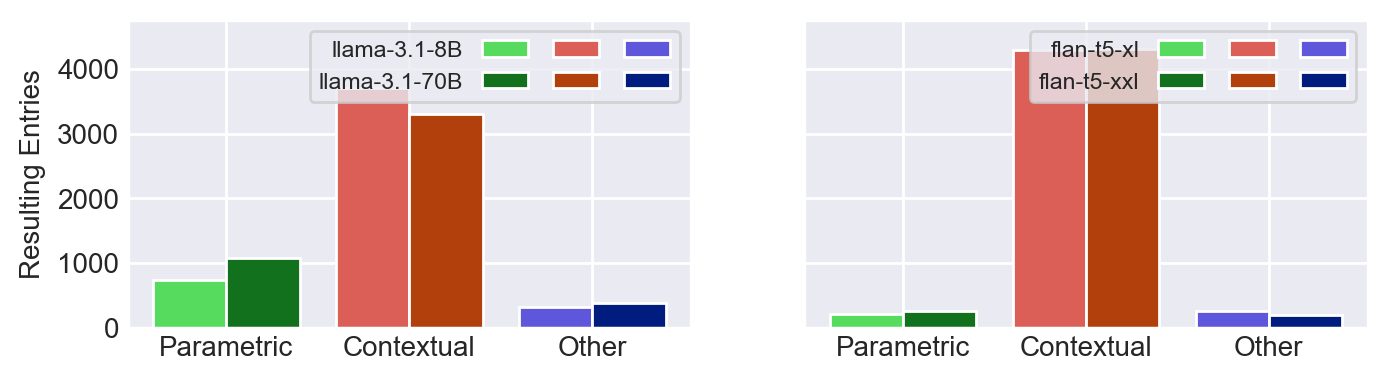
\includegraphics[width=\columnwidth]{both_amount.png}
	\caption{Amount of each answers of each category when running a context with counterparametric information for encoder-decoder and Decoder-only models of different sizes.}
	\label{total_plot}
\end{figure}

\begin{table*}[t]
	\centering
	\footnotesize
	\begin{tabular}{>{\bfseries}l | r r r | r r r | r r r | r r r}
		\toprule
			& \multicolumn{3}{c|}{\smallflan{}} & \multicolumn{3}{c|}{\bigflan{}} & \multicolumn{3}{c|}{\texttt{llama-8B}} & \multicolumn{3}{c}{\texttt{llama-70B}}  \\
			& \Pc{} & \Cc{} & \Oc{} & \Pc{} & \Cc{} & \Oc{} & \Pc{} & \Cc{} & \Oc{} & \Pc{} & \Cc{} & \Oc{}  \\
		\midrule
			Person           &  32 &  900 & 37 &  23 &  890 & 56 &  40 &  833 & 96 & 209 & 614 & 146 \\
			City             & 120 & 1030 & 40 &  78 & 1093 & 19 & 117 & 1007 & 66 & 166 & 966 &  58 \\
			Principle        &  13 &  164 &  8 &   9 &  168 &  8 &  44 &  118 & 23 &  44 & 117 &  24 \\
			Element          &   6 &  637 &  2 & 102 &  515 & 28 & 218 &  385 & 42 & 275 & 347 &  23 \\
			Book             &  26 &  488 & 25 &  18 &  457 & 64 & 135 &  344 & 60 & 154 & 318 &  67 \\
			Painting         &  26 &  446 & 56 &   4 &  498 & 26 &  47 &  458 & 23 &  49 & 445 &  34 \\
			Historical Event &  11 &  217 & 28 &   1 &  254 &  1 &  81 &  154 & 21 & 117 & 118 &  21 \\
			Building         &  14 &  174 & 10 &   0 &  189 &  9 &  27 &  163 &  8 &  31 & 159 &   8 \\
			Composition      &   0 &  228 & 22 &   7 &  240 &  3 &  36 &  200 & 14 &  25 & 219 &   6 \\
		\bottomrule \addlinespace[4pt]
	\end{tabular}
	\caption{Results for each model tested on queries with counterparametric context in each one of the 10 given categories.}
	\label{cats_table}
\end{table*}
